% \def\tendethi{ĐỀ MINH HOẠ 2025}
\begin{name}
    {\tenchude}
    {ĐỀ MINH HOẠ 2025}
    {\tentruong}
    {\thoigian}
\end{name}

\Opensolutionfile{ansbook}[ans/ansbook-DE-PNL-1-MH]
\TN
\Opensolutionfile{ans}[ans/ans-DE-PNL-01-T]


%%==========Câu 1
\begin{ex}%[Đề Minh Hoạ TNTHPT 2024-2025]%[2PhatTrien-DMH-2024-2025, GV: Hoàng Trọng Tấn]%[2D4N1-4]
    Nguyên hàm của hàm số $f(x) = \mathrm{e}^x$ là:
    \choice
    {$\dfrac{\mathrm{e}^{x+1}}{x+1} + C$}
    {\True $\mathrm{e}^x + C$}
    {$\dfrac{\mathrm{e}^x}{x} + C$}
    {$x \mathrm{e}^{x-1} + C$}
    \loigiai{
        Nguyên hàm của $f(x)=\mathrm{e}^x$ là $F(x)=\mathrm{e}^x+C$.	
    }
\end{ex}

%%==========Câu 2
\begin{ex}%[Đề Minh Hoạ TNTHPT 2024-2025]%[2PhatTrien-DMH-2024-2025, GV: Hoàng Trọng Tấn]%[2D4N3-3]
    Cho hàm số $y = f(x)$ liên tục, nhận giá trị dương trên đoạn $[a;b]$. Xét hình phẳng $(H)$ giới hạn bởi đồ thị hàm số $y = f(x)$, trục hoành và hai đường thẳng $x = a$, $x = b$. Khối tròn xoay được tạo thành khi quay hình phẳng $(H)$ quanh trục $Ox$ có thể tích là:
    \choice
    {$V = \pi \displaystyle \int_a^b [f(x)] \mathrm{\,d}x$}
    {$V = \pi^2 \displaystyle \int_a^b f(x) \mathrm{\,d}x$}
    {$V = \pi^2 \displaystyle \int_a^b [f(x)]^2 \mathrm{\,d}x$}
    {\True $V = \pi \displaystyle \int_a^b [f(x)]^2 \mathrm{\,d}x$}
    \loigiai{
        Khối tròn xoay được tạo thành khi quay hình phẳng $(H)$ quanh trục $Ox$ có thể tích là $V = \pi \displaystyle \int_a^b [f(x)]^2 \mathrm{\,d}x$.
    }
\end{ex}

%%==========Câu 3
\begin{ex}%[Đề Minh Hoạ TNTHPT 2024-2025]%[2PhatTrien-DMH-2024-2025, GV: Hoàng Trọng Tấn]%[2D3H2-1]
    Hai mẫu số liệu ghép nhóm $M_1$, $M_2$ có bảng tần số ghép nhóm như sau:
    \begin{center}
        \begin{tabular}{|c|c|c|c|c|c|}
            \hline
            Nhóm & $[8;10)$ & $[10;12)$ & $[12;14)$ & $[14;16)$ & $[16;18)$ \\
            \hline
            $M_1$ & $3$ & $4$ & $8$ & $6$ & $4$ \\
            \hline
            $M_2$ & $6$ & $8$ & $16$ & $12$ & $8$ \\
            \hline
        \end{tabular}
    \end{center}	
    Gọi $s_1$, $s_2$ lần lượt là độ lệch chuẩn của mẫu số liệu ghép nhóm $M_1$, $M_2$. Phát biểu nào sau đây là đúng?
    \choice
    {\True $s_1 = s_2$}
    {$s_1 = 2s_2$}
    {$2s_1 = s_2$}
    {$4s_1 = s_2$}
    \loigiai{
        Giá trị trung bình của mẫu $M_1$:
        $$
        \overline{x}_1 = \dfrac{9 \cdot 3 + 11 \cdot 4 + 13 \cdot 8 + 15 \cdot 6 + 17 \cdot 4}{3 + 4 + 8 + 6 + 4}
        = \dfrac{333}{25} = 13{,}32
        $$	
        Tính các sai lệch bình phương:
        $$
        (9 - 13{,}32)^2 = 18{,}6624,  (11 - 13{,}32)^2 = 5{,}3824, (13 - 13{,}32)^2 = 0{,}1024, 
        $$
        $$
        (15 - 13{,}32)^2 = 2{,}8224, (17 - 13{,}32)^2 = 13{,}5424
        $$
        Phương sai của mẫu $M_1$:
        $$
        s_1^2 = \dfrac{3\cdot 18{,}6624 + 4\cdot 5{,}3824 + 8\cdot 0{,}1024 + 6\cdot 2{,}8224 + 4\cdot 13{,}5424}{25}=5{,}9776
        $$
        Vậy, độ lệch chuẩn của mẫu $M_1$ là:
        $$
        s_1 = \sqrt{5{,}9776} \approx 2{,}445
        $$
        Tương tự 
        \\
        Giá trị trung bình của mẫu $M_2$:
        $$
        \overline{x}_2 = \dfrac{9 \cdot 6 + 11 \cdot 8 + 13 \cdot 16 + 15 \cdot 12 + 17 \cdot 8}{6 + 8 + 16 + 12 + 8}
        = \dfrac{666}{50} = 13{,}32
        $$	
        Tính các sai lệch bình phương:
        $$
        (9 - 13{,}32)^2 = 18{,}6624, \quad (11 - 13{,}32)^2 = 5{,}3824, \quad (13 - 13{,}32)^2 = 0{,}1024,
        $$
        $$
        (15 - 13{,}32)^2 = 2{,}8224, \quad (17 - 13{,}32)^2 = 13{,}5424
        $$
        Phương sai của mẫu $M_2$:
        $$
        s_2^2 = \dfrac{6\cdot 18{,}6624 + 8\cdot 5{,}3824 + 16\cdot 0{,}1024 + 12\cdot 2{,}8224 + 8\cdot 13{,}5424}{50}= 5{,}9776
        $$
        
        Vậy, độ lệch chuẩn của mẫu $M_2$ là:
        $$
        s_2 = \sqrt{5{,}9776} \approx 2{,}445
        $$
        \\
        Cả hai mẫu $M_1$ và $M_2$ đều có độ lệch chuẩn bằng nhau:
        $$
        s_1 = s_2 \approx 2{,}445
        $$
    }
\end{ex}

%%==========Câu 4
\begin{ex}%[Đề Minh Hoạ TNTHPT 2024-2025]%[2PhatTrien-DMH-2024-2025, GV: Hoàng Trọng Tấn]%[2H5N2-3]
    Trong không gian với hệ trục tọa độ $Oxyz$, phương trình của đường thẳng đi qua điểm $M(1;-3;5)$ và có một vectơ chỉ phương $\overrightarrow{u}(2;-1;1)$ là:
    \choice
    {$\dfrac{x-1}{2} = \dfrac{y+3}{-1} = \dfrac{z-5}{1}$}
    {$\dfrac{x+1}{2} = \dfrac{y+3}{-1} = \dfrac{z+5}{1}$}
    {\True $\dfrac{x-1}{2} = \dfrac{y+3}{1} = \dfrac{z-5}{-1}$}
    {$\dfrac{x+1}{2} = \dfrac{y+3}{-1} = \dfrac{z-5}{-1}$}
    \loigiai{
        Phương trình của đường thẳng đi qua điểm $M(1;-3;5)$ và có một vectơ chỉ phương $\overrightarrow{u}(2;-1;1)$ là $\dfrac{x-1}{2} = \dfrac{y+3}{1} = \dfrac{z-5}{-1}$.
    }
\end{ex}

%%==========Câu 5
\begin{ex}%[Đề Minh Hoạ TNTHPT 2024-2025]%[2PhatTrien-DMH-2024-2025, GV: Hoàng Trọng Tấn]%[2D1N4-1]
    %[id6]
    \immini{
        Cho hàm số $y = \dfrac{ax + b}{cx + d}$ ($c \neq 0$, $ad - bc \neq 0$) có đồ thị như hình vẽ bên. Tiệm cận ngang của đồ thị hàm số là:
        \choice
        {$x = -1$}
        {\True $y = \dfrac{1}{2}$}
        {$y = -1$}
        {$x = \dfrac{1}{2}$}
    }
    {
        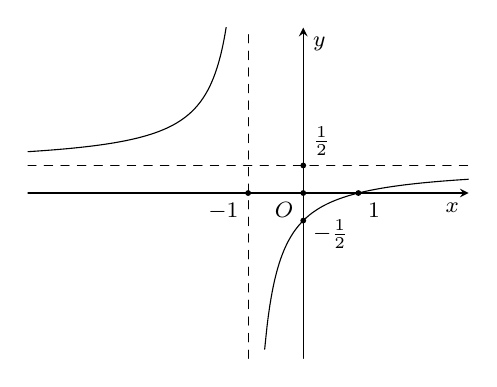
\begin{tikzpicture}[line join = round, line cap=round,>=stealth,font=\footnotesize,scale=0.7]
            \clip (-5,-3) rectangle (3,3);
            \draw[smooth,samples=100,domain=-0.7:4] plot(\x,{
                ((\x)-1)/(2*(\x)+2)
            });
            \draw[smooth,samples=100,domain=-5:-1.1] plot(\x,{
                ((\x)-1)/(2*(\x)+2)
            });
            \draw[->] (0,-3)--(0,3) node[below right]{$y$};
            \draw[->] (-5,0)--(3,0) node[below left]{$x$};
            \draw[dashed] 
            (-1,-3)--(-1,3)(-5,0.5)--(5,0.5)
            ;
            \fill 
            (0,0) circle(1.5pt) node[below left]{$O$}
            (0,0.5) circle(1.5pt) node[above right]{$\frac{1}{2}$}
            (-1,0) circle(1.5pt) node[below left]{$-1$}
            (1,0) circle(1.5pt) node[below right]{$1$}
            (0,-0.5) circle(1.5pt) node[right,yshift=-5pt]{$-\frac{1}{2}$}
            ;
        \end{tikzpicture}
    }
    \loigiai{ 
        Dựa vào hình vẽ bên ta thấy đường tiệm cận ngang của đồ thị hàm là $y=\dfrac{1}{2}$.
    }
\end{ex}


%%==========Câu 6
\begin{ex}%[Đề Minh Hoạ TNTHPT 2024-2025]%[2PhatTrien-DMH-2024-2025, GV: Hoàng Trọng Tấn]%[1D6N4-3]
    Tập nghiệm của bất phương trình $\log_2 (x-1) < 3$ là:
    \choice
    {\True $(1;9)$}
    {$(-\infty;9)$}
    {$(9; +\infty)$}
    {$(1;7)$}
    \loigiai{
        Ta có $\log_2 (x-1) < 3\Leftrightarrow \log_2(x-1)< \log_2 8\Leftrightarrow 0<x-1<8\Leftrightarrow 1<x<9$.
    }
\end{ex}

%%==========Câu 7
\begin{ex}%[Đề Minh Hoạ TNTHPT 2024-2025]%[2PhatTrien-DMH-2024-2025, GV: Hoàng Trọng Tấn]%[2H5N1-2]
    Trong không gian với hệ trục tọa độ $Oxyz$, cho mặt phẳng $(P)$ có phương trình $x - 3y - z + 8 = 0$. Véctơ nào sau đây là một vectơ pháp tuyến của mặt phẳng $(P)$?
    \choice
    {$\overrightarrow{n}_1(1;-3;1)$}
    {\True $\overrightarrow{n}_2(1;-3;-1)$}
    {$\overrightarrow{n}_3(1;3;8)$}
    {$\overrightarrow{n}_4(1;3;8)$}
    \loigiai{
        Véctơ $\overrightarrow{n}_2(1;-3;-1)$ là một vectơ pháp tuyến của mặt phẳng $(P)$.
    }
\end{ex}

%%==========Câu 8
\begin{ex}%[Đề Minh Hoạ TNTHPT 2024-2025]%[2PhatTrien-DMH-2024-2025, GV: Hoàng Trọng Tấn]%[1H8N4-2]
    Cho hình chóp $S.ABCD$ có đáy $ABCD$ là hình chữ nhật và $SA \perp (ABCD)$. Mặt phẳng nào sau đây vuông góc với mặt phẳng $(ABCD)$?
    \choice
    {\True $(SAB)$}
    {$(SBC)$}
    {$(SCD)$}
    {$(SBD)$}
    \loigiai{
        Ta có $SA\subset (SAB)$ và $SA \perp (ABCD)\Rightarrow (SAB)\perp (ABCD)$.
    }
\end{ex}

%%==========Câu 9
\begin{ex}%[Đề Minh Hoạ TNTHPT 2024-2025]%[2PhatTrien-DMH-2024-2025, GV: Hoàng Trọng Tấn]%[1D6N4-2]
    Nghiệm của phương trình $2^x = 6$ là:
    \choice
    {$x = \log_2 2$}
    {$x = 3$}
    {$x = 4$}
    {\True $x = \log_2 6$}
    \loigiai{
        Ta có $2^x = 6\Leftrightarrow x=\log_2 6$.	
    }
\end{ex}

%%==========Câu 10
\begin{ex}%[Đề Minh Hoạ TNTHPT 2024-2025]%[2PhatTrien-DMH-2024-2025, GV: Hoàng Trọng Tấn]%[1D2N1-3]
    Cấp số cộng $(u_n)$ có $u_1 = 1$ và $u_2 = 3$. Số hạng $u_5$ của cấp số cộng là:
    \choice
    {$5$}
    {$7$}
    {\True $9$}
    {$11$}
    \loigiai{
        Ta có công sai $d=u_2-u_1=2$.
        \\
        Suy ra $u_5=u_1+4d\Leftrightarrow u_5=1+4\cdot 2=9$.	
    }
\end{ex}

%%==========Câu 11
\begin{ex}%[Đề Minh Hoạ TNTHPT 2024-2025]%[2PhatTrien-DMH-2024-2025, GV: Hoàng Trọng Tấn]%[2H2H1-2]
    
    \immini{
        Cho hình hộp $ABCDA'B'C'D'$ (minh họa như hình bên). Phát biểu nào sau đây là đúng?
        \choice
        {$\overrightarrow{AB} + \overrightarrow{BB'} + \overrightarrow{B'A'} = \overrightarrow{AC'}$}
        {$\overrightarrow{AB} + \overrightarrow{BC} + \overrightarrow{C'D'} = \overrightarrow{AC'}$}
        {$\overrightarrow{AB} + \overrightarrow{AC} + \overrightarrow{AA'} = \overrightarrow{AC'}$}
        {\True $\overrightarrow{AB} + \overrightarrow{AA'} + \overrightarrow{AD} = \overrightarrow{AC'}$}
    }
    {
        \begin{tikzpicture}[line join = round, line cap=round,>=stealth,font=\footnotesize,scale=0.7]
            \def\r{3}
            \path 
            (0,0) coordinate (A)
            (4,0) coordinate (D)
            (-2,-2) coordinate (B)
            ($(B)+(D)-(A)$) coordinate (C)
            ($(A)+(1,\r)$) coordinate (A')
            ($(B)+(1,\r)$) coordinate (B')
            ($(C)+(1,\r)$) coordinate (C')
            ($(D)+(1,\r)$) coordinate (D')
            ;
            
            \draw (B)--(C)--(D)--(D')--(A')--(B')--(B)
            (B')--(C')--(D') (C)--(C')
            ;
            \draw[dashed]
            (B)--(A)--(D) (A)--(A') (A)--(C');
            \foreach \p/\r in {A/-90,B/-90,C/-90,D/-90,A'/90,B'/90,C'/90,D'/90}
            \fill (\p) circle (1.2pt) node[shift={(\r:3mm)}]{$\p$};
        \end{tikzpicture}
    }
    \loigiai{
        Ta có $\overrightarrow{AB}+\overrightarrow{AD}=\overrightarrow{AC}$.
        \\
        Suy ra $\overrightarrow{AB} + \overrightarrow{AA'} + \overrightarrow{AD} = \overrightarrow{AC}+\overrightarrow{AA'}=\overrightarrow{AC'}$.
    }
\end{ex}

%%==========Câu 12
\begin{ex}%[Đề Minh Hoạ TNTHPT 2024-2025]%[2PhatTrien-DMH-2024-2025, GV: Hoàng Trọng Tấn]%[2D1N1-2]
    \immini{
        Cho hàm số có đồ thị như hình vẽ bên. Hàm số đã cho đồng biến trên khoảng nào sau đây?
        \choice
        {$(-\infty;1)$}
        {$(-\infty;-1)$}
        {\True $(-1;1)$}
        {$(1;+ \infty)$}	
    }
    {
        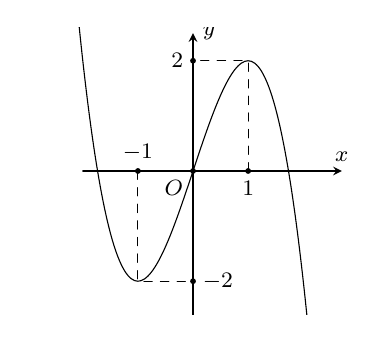
\begin{tikzpicture}[line join = round, line cap=round,>=stealth,font=\footnotesize,scale=0.7]
            \clip (-3,-2.6) rectangle (3,2.6);
            \draw[smooth,samples=100,domain=-3:3] plot(\x,{
                -(\x)^3+3*(\x)
            });
            \draw[->] (-2,0)--(2.7,0) node[above]{$x$};
            \draw[->] (0,-3)--(0,2.5) node[right]{$y$};
            \fill(0,0) circle(1.5pt) node[below left]{$O$};
            \fill 
            (1,0) circle(1.5pt) node[below]{$1$}
            (-1,0) circle(1.5pt) node[above]{$-1$}
            (0,2) circle(1.5pt) node[left]{$2$}
            (0,-2) circle(1.5pt) node[right]{$-2$}
            ;
            \draw[dashed] 
            (-1,0)--(-1,-2)--(0,-2)
            (1,0)--(1,2)--(0,2)
            ;
        \end{tikzpicture}
    }
    \loigiai{
        Quan sát hình vẽ từ trái sang phải ta thấy hình vẽ hướng lên, trên khoảng $(-1;1)$.
        \\
        Suy ra hàm số đã cho đồng biến trên $(-1;1)$.
    }
\end{ex}

\Closesolutionfile{ans}
\TNTF
\Opensolutionfile{ans}[ans/ans-DE-PNL-01-TF]




%%==========Câu 13
\begin{ex}%[Đề Minh Hoạ TNTHPT 2024-2025]%[2PhatTrien-DMH-2024-2025, GV: Hoàng Trọng Tấn]%[2D1H3-1]
    Cho hàm số $f(x) = 2\cos x + x$
    \choiceTF
    {\True $f(0) = 2$; $f\left(\dfrac{\pi}{2}\right) = \dfrac{\pi}{2}$}
    {$f'(x) = 2\sin x + 1$}
    {\True $f'(x) = 0$ có nghiệm trên đoạn $\left[0; \dfrac{\pi}{2}\right]$ là $\dfrac{\pi}{6}$}
    {\True Giá trị lớn nhất của $f(x)$ trên đoạn $\left[0; \dfrac{\pi}{2}\right]$ là $\sqrt{3} + \dfrac{\pi}{6}$}
    \loigiai{
        
        \begin{itemchoice}	
            \itemch \textbf{Đúng.}\\	Ta có $f(0)=2\cos 0 +0 =2$ và $f\left(\dfrac{\pi}{2}\right)=2\cdot 0+\dfrac{\pi}{2}$.
            \itemch \textbf{Sai.} \\	$f'(x)=-2\sin x +1$.
            \itemch  \textbf{Đúng.} \\	$f'(x)=0\Leftrightarrow -2\sin x +1 =0 \Leftrightarrow \sin x=\dfrac{1}{2}$.
            \\
            Mà $x\in \left[0;\dfrac{\pi}{2}\right]\Rightarrow x=\dfrac{\pi}{6}$.
            \itemch \textbf{Đúng.} \\Ta có $f\left(\dfrac{\pi}{6}\right)=\sqrt{3}+\dfrac{\pi}{6}>2$.
            Suy ra $\max\limits_{[0;\tfrac{\pi}{2}]}=\sqrt{3}+\dfrac{\pi}{6}$.
        \end{itemchoice}
    }
\end{ex}



%%==========Câu 14
\begin{ex}%[Đề Minh Hoạ TNTHPT 2024-2025]%[2PhatTrien-DMH-2024-2025, GV: Hoàng Trọng Tấn]%[2D4V2-6]
    Một người điều khiển ô tô đang ở đường dẫn muốn nhập làn vào đường cao tốc. Khi ô tô cách điểm nhập làn $200$ m, tốc độ của ô tô là $36$ km/h. Hai giây sau đó, ô tô bắt đầu tăng tốc với tốc độ $v(t) = at + b$ ($a$, $b \in \mathbb{R}$, $a > 0$), trong đó $t$ là thời gian tính bằng giây kể từ khi bắt đầu tăng tốc. Biết rằng ô tô nhập làn cao tốc sau $12$ giây và duy trì sự tăng tốc trong $24$ giây kể từ khi bắt đầu tăng tốc.
    \choiceTF
    {\True Quãng đường ô tô đi được từ khi bắt đầu tăng tốc đến khi nhập làn là $180$ m}
    {\True Giá trị của $b$ là $10$}
    {Quãng đường $S(t)$ (đơn vị: mét) mà ô tô đi được trong thời gian $t$ giây ($0 \leq t \leq 24$) kể từ khi tăng tốc được tính theo công thức $S(t) =\displaystyle \int_0^{24} v(t) \mathrm{\,d}t$}
    {Sau $24$ giây kể từ khi tăng tốc, tốc độ của ô tô không vượt quá tốc độ tối đa cho phép là $100$ km/h}
    \loigiai{
        \begin{center}
            \begin{tikzpicture}[line join = round, line cap=round,>=stealth,font=\footnotesize,scale=1]
                \draw 
                (0,0)node[above]{$A$} node[yshift=25pt,pos=0.5]{$v_0=36$ km/h}
                -- (3,0)node[above]{$B$} node[yshift=-10pt,pos=0.5]{$2$ giây} 
                node[xshift=20pt,yshift=25pt]{$v(t)=at+b$ (m/s)}--(8,0) node[above]{$C$}--(14,0) node[above]{$D$}
                ;
                \draw[<->] (3,-0.75)--(8,-0.75) node[below,pos=0.5]{$12$ giây}	;
                \draw[<->] (3,-1.5)--(14,-1.5) node[below,pos=0.5]{$24$ giây}	;
                %\draw[<->] (0,-2.5)--(3,-2.5) node[below,pos=0.5]{$S_1$ m}	;
                \draw[<->] (0,-2.5)--(8,-2.5) node[below,pos=0.5]{$200$ m}	;
            \end{tikzpicture}
        \end{center}
        
        \begin{itemchoice}
            \itemch \textbf{Đúng.}	\\ 
            Đổi đơn vị $36$ km/h bằng $10$ m/s.
            \\
            Quãng đường ô tô đi được $2$ giây đầu là $AB=10\cdot 2=20$ m. 
            \\
            Quãng đường ô tô đi được từ khi bắt đầu tăng tốc đến khi nhập làn là $BC=AC-AB=200-20=180$ m.
            
            \itemch \textbf{Đúng.}\\
            Khi $t=0$ thì $v_t=v_o=10\Rightarrow 10=a\cdot 0 +b\Rightarrow b=10$.
            
            \itemch\textbf{Sai.}\\
            Quãng đường đi được trong $t$ giây là $S(t)-S(0)=\displaystyle \int_0^t v(t) \mathrm{\,d}t$.
            
            \itemch \textbf{Sai.}
            \\
            Ta có $v(t)=at+10$.	Lại có 
            \begin{eqnarray*}
                BC=\displaystyle\int_0^{12} (at+10) \mathrm{\,d}t
                &\Leftrightarrow&	\left( \dfrac{at^2}{2}+10t\right)\Bigg|_0^{12}=180
                \\
                &\Leftrightarrow& 72a+120=180
                \\
                &\Leftrightarrow& a=\dfrac{5}{6}
            \end{eqnarray*}
            Vậy $v(t)=\dfrac{5}{6}t +10 \Rightarrow v(24)=30$ m/s $=108$ km/h. 
        \end{itemchoice}
    }
\end{ex}



%%==========Câu 15
\begin{ex}%[Đề Minh Hoạ TNTHPT 2024-2025]%[2PhatTrien-DMH-2024-2025, GV: Hoàng Trọng Tấn]%[2D6V2-3]
    Trước khi đưa một loại sản phẩm ra thị trường, người ta đã phỏng vấn ngẫu nhiên $200$ khách hàng về sản phẩm đó. Kết quả thống kê như sau: có $105$ người trả lời 
    \lq\lq  sẽ mua\rq\rq; có $95$ người trả lời \lq\lq  không mua\rq\rq.
    Kinh nghiệm cho thấy tỉ lệ khách hàng thực sự sẽ mua sản phẩm tương ứng với những câu trả lời \lq\lq  sẽ mua\rq\rq\, và \lq\lq  không mua\rq\rq\, lần lượt là $70\%$ và $30\%$. Gọi $A$ là biến cố \lq\lq  Người được phỏng vấn thực sự sẽ mua sản phẩm\rq\rq. Gọi $B$ là biến cố \lq\lq  Người được phỏng vấn trả lời sẽ mua sản phẩm\rq\rq.
    \choiceTF
    {\True $\mathrm{P}(B) = \dfrac{21}{40}$ và $\mathrm{P}(\overline{B}) = \dfrac{19}{40}$}
    {$\mathrm{P}(A \mid B) = 0{,}3$}
    {\True $\mathrm{P}(A) = 0{,}51$}
    {Trong số những người được phỏng vấn thực sự sẽ mua sản phẩm có $70\%$ người đã trả lời \lq\lq  sẽ mua\rq\rq\, khi được phỏng vấn (kết quả tính theo phần trăm được làm tròn đến hàng đơn vị)}
    \loigiai{			
        \begin{itemchoice}
            \itemch \textbf{Đúng}.\\
            Xác suất người được phỏng vấn thực sự sẽ mua sản phẩm $B$ và không mua sản phẩm $\overline{B} $ được cho như sau:
            $\mathrm{P}(B) = \dfrac{105}{200}=\dfrac{21}{40}$, $\mathrm{P}(\overline{B}) =1-\dfrac{21}{40}=\dfrac{19}{40}$.
            
            \itemch \textbf{Sai.}\\
            $\mathrm{P}(A\mid B)$ là xác suất có điều kiện, mô tả xác suất một người thực sự sẽ mua sản phẩm (biến cố $A$) khi biết rằng người đó đã trả lời \lq\lq  sẽ mua\rq\rq\, trong cuộc phỏng vấn (biến cố $B$).
            \\
            Vậy $\mathrm{P}(A\mid B)=70\%=0{,}7$.
            
            \itemch \textbf{Đúng.}\\
            Từ $\mathrm{P}(A\mid B)=0{,}7\Rightarrow P(A\mid \overline{B})=1-0{,}7=0{,}3$.
            \\
            Áp dụng công thức xác suất toàn phần ta có 
            $$
            \mathrm{P}(A) = \mathrm{P}(A \mid B) \cdot \mathrm{P}(B) + \mathrm{P}(A \mid \overline{B}) \cdot \mathrm{P}(\overline{B})=0{,}7 \cdot \dfrac{21}{40} + 0{,}3 \cdot \dfrac{19}{40}=0{,}51.
            $$
            
            \itemch \textbf{Sai.}\\
            Phát biểu này yêu cầu tính xác suất có điều kiện $\mathrm{P}(B\mid A)$, tức là xác suất một người đã trả lời \lq\lq  sẽ mua\rq\rq\, khi biết rằng người đó thực sự sẽ mua sản phẩm.
            \\
            Để tính $\mathrm{P}(B \mid A)$, ta áp dụng định lý Bayes:
            \begin{eqnarray*}
                && \mathrm{P}(B \mid A) = \dfrac{\mathrm{P}(A \mid B) \cdot \mathrm{P}(B)}{\mathrm{P}(A)}
                \\
                &\Leftrightarrow& \mathrm{P}(B \mid A) = \dfrac{0{,}7 \cdot \dfrac{21}{40}}{0{,}51}\approx 0{,}72=72\%.
            \end{eqnarray*}
            
        \end{itemchoice}
        
    }
\end{ex}

%%==========Câu 16
\begin{ex}%[Đề Minh Hoạ TNTHPT 2024-2025]%[2PhatTrien-DMH-2024-2025, GV: Hoàng Trọng Tấn]%[id6]
    \immini{
        Các thiên thạch có đường kính lớn hơn $140$ m và có thể lại gần Trái Đất ở khoảng cách nhỏ hơn $7\,500\,000$ km được coi là những vật thể có khả năng va chạm gây nguy hiểm cho Trái Đất. Để theo dõi những thiên thạch này, người ta đã thiết lập các trạm quan sát các vật thể bay gần Trái Đất. Giả sử có một hệ thống quan sát có khả năng theo dõi các vật thể ở độ cao không vượt quá $6\,600$ km so với mực nước biển. Coi Trái Đất là khối cầu có bán kính $6\,400$ km. Chọn hệ trục tọa độ $Oxyz$ trong không gian có gốc $O$ tại tâm Trái Đất và đơn vị độ dài trên mỗi trục tọa độ là $1\,000$ km. Một thiên thạch (coi như một hạt) chuyển động với tốc độ không đổi theo một đường thẳng từ điểm $M(6;20;0)$ đến điểm $N(-6;-12;16)$.
        
    }
    {
        \begin{tikzpicture}[line join = round, line cap=round,>=stealth,font=\footnotesize,transform shape,scale=0.8]
            \draw 
            (0,0) circle(3.5cm)
            ;
            \draw[fill=black!30] 
            (0,0) circle(1.6cm);
            \draw[<->] (0:3.5)--(0:1.6) node[pos=0.5,above]{$6\, 600$ km};
            \draw[<->] (0:0)--(0:1.6) node[pos=0.5,above]{$6\, 400$ km};
            \draw (130:3.5)coordinate (A)--(40:3.5)coordinate (B);
            \draw ($(A)!-0.4!(B)$) --(A)
            ($(A)!1.4!(B)$)--(B)
            ;
            
            \fill 
            (A)circle(1.5pt)node[above left]{$A$}
            (B)circle(1.5pt)node[above right]{$B$}
            ($(A)!-0.4!(B)$) circle(1.5pt)node[above]{$M$}
            ($(A)!1.4!(B)$)circle(1.5pt)node[above]{$N$}
            ;
            
        \end{tikzpicture}
    }
    \choiceTF
    {\True Đường thẳng $MN$ có phương trình tham số là $\heva{&x = 6 + 3t \\& y = 20 + 8t \\& z = -4t}$, $(t \in \mathbb{R})$}
    {Vị trí đầu tiên thiên thạch đi chuyển vào phạm vi theo dõi của hệ thống quan sát là điểm $A(-3; -4; 12)$}
    {\True Khoảng cách giữa vị trí đầu tiên và vị trí cuối cùng mà thiên thạch di chuyển trong phạm vi theo dõi của hệ thống quan sát  là $18\,900$ km (kết quả làm tròn đến hàng trăm đơn vị ki-lô-mét)}
    {\True Nếu thời gian di chuyển của thiên thạch trong phạm vi theo dõi của hệ thống quan sát là $3$ phút thì thời gian nó di chuyển từ $M$ đến $N$ là $6$ phút}
    \loigiai{
        \begin{itemchoice}
            \itemch \textbf{Đúng}.\\
            Ta có $\overrightarrow{MN}=(-12;-32;16)=-4\cdot (3;8;-4)$.
            \\
            Suy ra $MN$ có một véctơ chỉ phương là $\overrightarrow{u}=(3;8;-4)$.
            \\
            Phương trình tham số của đường thẳng $MN$ là $\heva{&x = 6 + 3t \\& y = 20 + 8t \\& z = -4t}$, $(t \in \mathbb{R})$.
            
            \itemch \textbf{Sai.}\\
            \begin{center}
                \begin{tikzpicture}[line join = round, line cap=round,>=stealth,font=\footnotesize,transform shape,scale=0.7]
                    \draw 
                    (0,0)coordinate (O) circle(3.5cm)
                    ;
                    \draw[fill=black!30] 
                    (0,0) circle(1.6cm);
                    \draw[<->] (0:3.5)--(0:1.6) node[pos=0.5,above]{$6\, 600$ km};
                    \draw[<->] (0:0)--(0:1.6) node[pos=0.5,above]{$6\, 400$ km};
                    \draw (130:3.5)coordinate (A)--(40:3.5)coordinate (B);
                    \path (0,0) node{\hypersetup{hidelinks}\href{HWKJsE1}{ }};
                    \draw ($(A)!-0.4!(B)$) --(A)
                    ($(A)!1.4!(B)$)--(B)
                    ;
                    
                    \fill 
                    (A)circle(1.5pt)node[above left]{$A$}
                    (B)circle(1.5pt)node[above right]{$B$}
                    ($(A)!-0.4!(B)$)coordinate (M) circle(1.5pt) circle(1.5pt)node[above]{$M$}
                    ($(A)!1.4!(B)$) node[above]{$N$}
                    ;
                    \draw 
                    (O)--($(A)!1/2!(B)$)coordinate(H) 
                    (O)--(A)
                    (O)--(M)
                    ; 
                    
                    
                    \foreach \p/\r in {O/-90,H/90}
                    \fill (\p) circle (1.2pt) node[shift={(\r:3mm)}]{$\p$};			
                    
                    \draw pic[draw,angle radius=3mm] {right angle = O--H--A}; 
                    
                \end{tikzpicture}
            \end{center}
            Do $H\in MN\Rightarrow H(6+3t;20+8t;-4t)$ suy ra $\overrightarrow{OH}=(6+3t;20+8t;-4t)$ 
            \\
            Hơn nữa
            \begin{eqnarray*}
                OH\perp MN &\Leftrightarrow& \overrightarrow{OH}\cdot \overrightarrow{u}=0
                \\
                &\Leftrightarrow& 3(6 + 3t) + 8(20 + 8t) + (-4)\cdot (-4t)=0
                \\
                &\Leftrightarrow&178 + 89t=0 \Leftrightarrow t=-2.
            \end{eqnarray*}
            Suy ra $H(0;4;8)$ và độ dài của $OH=\sqrt{4^2+8^2}=4\sqrt 5$ (nghìn km).
            \\
            Xét tam giác $OMH$
            \\ 
            $OM=\sqrt{6^2+20^2+0}=2\sqrt{109}$ (nghìn km).
            \\
            Suy ra $MH=\sqrt{OM^2-OH^2}=\sqrt{436-80}=2\sqrt{89}$ (nghìn km).
            \\
            Xét tam giác $OAH$, ta có $OA=6\,400+6\,600=13$ (nghìn km).
            \\
            $AH=\sqrt{OA^2-OH^2}=\sqrt{169-80}=\sqrt{89}$ (nghìn km).
            \\
            Suy ra $MH=2AH$ hay $A$ là trung điểm $MH$.
            \\
            Vậy toạ độ $A(3;12;4)$.
            
            
            \itemch \textbf{Đúng.}
            \\
            Độ dài đoạn $AB=2AH=2\sqrt{89}\approx 18{,}87$ nghìn km tức là $AH=18\, 870$ km $\approx 18\, 900$ km.
            
            \itemch \textbf{Đúng.}
            \\
            Ta có $3$ phút bằng $\dfrac{1}{20}$ giờ và $3$ phút bằng $\dfrac{1}{10}$ giờ.
            \\
            Vận tốc của thiên thạch $v=\dfrac{AB}{\dfrac{1}{20}}=378\,000$ (km/h) $=378$ (nghìn km/h).
            \\
            Độ dài của $MN=2MH=4\sqrt{89}$ (nghìn km).
            \\
            Thời gian đi từ $M$ đến $N$ là $\dfrac{4\sqrt{89}}{378}\approx 0{,}1$ h bằng $6$ phút.
        \end{itemchoice}
    }
\end{ex}
\Closesolutionfile{ans}
\TNSA
\Opensolutionfile{ans}[ans/ans-DE-PNL-01-SA]


%%==========Câu 17
\begin{ex}%[Đề Minh Hoạ TNTHPT 2024-2025]%[2PhatTrien-DMH-2024-2025, GV: Hoàng Trọng Tấn]%[id6]
    Cho hình lăng trụ đứng $ABC.A'B'C'$ có $AB = 5$, $BC = 6$, $CA = 7$. Khoảng cách giữa hai đường thẳng $AA'$ và $BC$ bằng bao nhiêu? (làm tròn kết quả đến hàng phần mười)
    \shortans[]{$4{,}9$}
    \loigiai{
        \begin{center}
            \begin{tikzpicture}[line join = round, line cap=round,>=stealth,font=\footnotesize,scale=1]
                \def \dai{4} 
                \def\rong{-1}
                \def\cao{3}
                \path 
                (0,0) coordinate (A) 
                (\dai,0) coordinate (B)
                (\dai/3,\rong) coordinate (C)
                ($(A)+(0,\cao)$) coordinate (A')
                ($(B)+(0,\cao)$) coordinate (B')
                ($(C)+(0,\cao)$) coordinate (C')
                ($(C)!0.3!(B)$) coordinate (H)
                ;
                \draw 
                (A')--(B')--(C')--cycle
                (A')--(A) (B')--(B) (C')--(C)
                (A)--(C)--(B)
                ;
                \draw pic[draw,angle radius=3mm] {right angle = A--H--B}; 
                \draw[dashed] (A)--(B) (A)--(H);
                \foreach \p/\r in {A/-120,B/-40,C/-90,A'/120,B'/40,C'/90,H/-90}
                \fill (\p) circle (1.2pt) node[shift={(\r:3mm)}]{$\p$};
                
                
            \end{tikzpicture}
        \end{center}	
        Kẻ đường cao $AH$ của tam giác $ABC$.
        \\
        Suy ra $AH\perp BC$ hơn nữa $AA'\perp (ABC)$ mà $AH\subset (ABC)\Rightarrow AA'\perp AH$.
        \\
        Suy ra $AH$ là đoạn vuông góc chung của $AA'$ và $BC$ hay $d[AA',BC]=AH$.
        \\
        Nửa chu vi tam giác $ABC$ là $\mathrm{P}=\dfrac{5+6+7}{2}=9$.
        \\
        Áp dụng công thức Hê Rông ta có diện tích tam giác $ABC$ là
        $$
        S=\sqrt{p(p-5)(p-6)(p-7)}=6\sqrt 6.
        $$
        Suy ra độ dài đường cao $AH$ là $\dfrac{2\cdot 6\sqrt 6}{6}=2\sqrt 6\approx 4{,}9$.
    }
\end{ex}

%%==========Câu 18
\begin{ex}%[Đề Minh Hoạ TNTHPT 2024-2025]%[2PhatTrien-DMH-2024-2025, GV: Hoàng Trọng Tấn]%[id6]
    \immini{
        Một trò chơi điện tử quy định như sau: Có $4$ trụ $A$, $B$, $C$, $D$ với số lượng các thử thách trên đường đi giữa các cặp trụ được mô tả trong hình bên. Người chơi xuất phát từ một trụ nào đó, đi qua tất cả các trụ còn lại, mỗi khi đi qua một trụ thì trụ đó sẽ bị phá hủy và không thể quay trở lại trừ khi trò chơi kết thúc. Người chơi vẫn phải trở về trụ ban đầu. Tổng số thử thách của đường đi thỏa mãn điều kiện trên nhận giá trị nhỏ nhất là bao nhiêu?
    }
    {
        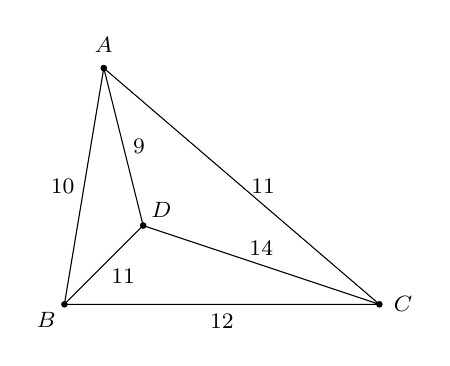
\begin{tikzpicture}[line join = round, line cap=round,>=stealth,font=\footnotesize,scale=1]
            \path 
            (0,0) coordinate (B)
            (0.5,3) coordinate (A)
            (4,0) coordinate (C)
            (1,1)coordinate (D)
            ;
            \draw (A)--(B)--(C)--cycle
            (A)--(D) (B)--(D) (C)--(D)
            ;
            \path 
            (A)--(B)node[left,pos=0.5]{$10$}
            (A)--(C)node[right,pos=0.5]{$11$}
            (C)--(B)node[below,pos=0.5]{$12$}
            (A)--(D)node[right,pos=0.5]{$9$}
            (B)--(D)node[below,xshift=7pt,yshift=2pt,pos=0.5]{$11$}
            (C)--(D)node[above,pos=0.5]{$14$}
            ;
            \foreach \p/\r in {A/90,B/-140,C/0,D/40}
            \fill (\p) circle (1.2pt) node[shift={(\r:3mm)}]{$\p$};
            
            
        \end{tikzpicture}
    }
    \shortans{$43$}
    \loigiai{
        Do $AD$ có $9$ thử thách là đường đi có số thử thách ít nhất nên ta sẽ bắt đầu từ $A$ đến $D$.
        \\
        Do $DB$ có $11$ thử thách và $DC$ có $14$ thử thách nên ta sẽ đi từ $D$ đến $B$.
        \\
        Lúc này trụ $A$ và $D$ đã bị phá huỷ nên ta đi từ $B$ đến $C$ với số thử thách là $12$.
        \\
        Cuối cùng đi từ $C$ đến $A$ với số thử thách là $11$.
        \\
        Vậy tổng cộng có $9+11+12+11=43$ thử thách.
    }
\end{ex}

%%==========Câu 19
\begin{ex}%[Đề Minh Hoạ TNTHPT 2024-2025]%[2PhatTrien-DMH-2024-2025, GV: Hoàng Trọng Tấn]%[id6]
    Hệ thống định vị toàn cầu GPS là một hệ thống cho phép xác định vị trí của một vật thể trong không gian. Trong cùng một thời điểm, vị trí của một điểm $M$ trong không gian sẽ được xác định bởi bốn vệ tinh cho trước nhờ các bộ thu phát tín hiệu đặt trên các vệ tinh. Giả sử trong không gian với hệ tọa độ $Oxyz$, có bốn vệ tinh lần lượt đặt tại các điểm $A(3;1;0)$, $B(3;6;6)$, $C(4;6;2)$, $D(6;2;14)$; vị trí $M(a;b;c)$ thỏa mãn $MA = 3$, $MB = 6$, $MC = 5$, $MD = 13$. Khoảng cách từ điểm $M$ đến điểm $O$ bằng bao nhiêu?
    \shortans{3}
    \loigiai{
        Giả sử $M(a;b;c)$. Ta có
        \begin{eqnarray*}
            MA=3&\Leftrightarrow& \sqrt{(a-3)^2+(b-1)^2+c^2}=3
            \\
            MB=6&\Leftrightarrow&\sqrt{(a-3)^2+(b-6)^2+(c-6)^2}=6
            \\
            MC=5&\Leftrightarrow&\sqrt{(a-4)^3+(b-6)^2+(c-2)^2}=5
            \\
            MD=13&\Leftrightarrow&\sqrt{(a-6)^3+(b-2)^2+(c-14)^2}=13
        \end{eqnarray*}
        Ta có hệ phương trình $\heva{
            & a^2 + b^2 + c^2 - 6a - 2b + 1 = 0\\
            & a^2 + b^2 + c^2 - 6a - 12b - 12c + 45 = 0 \\
            & a^2 + b^2 + c^2 - 8a - 12b - 4c + 31 = 0 \\
            & a^2 + b^2 + c^2 - 12a - 4b - 28c + 67 = 0.
        }$
        \\
        Giữ nguyên phương trình thứ nhất, lấy phương trình thứ nhất trừ vế theo vế với các phương trình còn lại ta được hệ phương trình mới như sau 
        \\
        $\heva{
            & a^2 + b^2 + c^2 - 6a - 2b + 1 = 0 \\
            & 10b + 12c = 44 \\
            & 2a + 10b + 4c = 30 \\
            & 6a + 2b + 28c = 66
        }\Leftrightarrow \heva{
            & a^2 + b^2 + c^2 - 6a - 2b + 1 = 0 \\
            & a = 1 \\
            & b = 2 \\
            & c = 2.
        }$
        \\
        Thế $a=1$, $b=2$, $c=2$ vào phương trình thứ nhất ta thấy thoả mãn. 
        \\
        Vậy điểm $M(1;2;2)\Rightarrow OM=\sqrt{1+4+4}=3$.
    }
\end{ex}

%%==========Câu 20
\begin{ex}%[Đề Minh Hoạ TNTHPT 2024-2025]%[2PhatTrien-DMH-2024-2025, GV: Hoàng Trọng Tấn]%[id6]
    \immini{
        Kiến trúc sư thiết kế một khu sinh hoạt cộng đồng có dạng hình chữ nhật với chiều rộng và chiều dài lần lượt là $60$ m và $80$ m. Trong đó, phần được tô màu đậm là sân chơi, phần còn lại để trồng hoa. Mỗi phần trồng hoa có đường biên cong là một phần của parabola với đỉnh thuộc một trục đối xứng của hình chữ nhật và có khoảng cách từ đường biên cong đến trục đối xứng bằng $20$ m (xem hình minh họa). Diện tích của phần sân chơi là bao nhiêu mét vuông?
    }
    {
        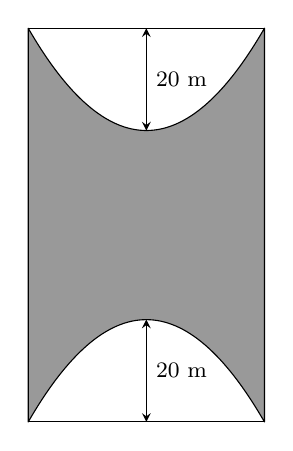
\begin{tikzpicture}[line join = round, line cap=round,>=stealth,font=\footnotesize,scale=1]
            \draw (0,0) rectangle (3,5);
            \draw[fill=black!40] (0,0)..controls +(60:2) and +(120:2)..(3,0)--(3,5)
            ..controls +(-120:2) and +(-60:2).. (0,5)--cycle
            ;
            
            \draw[<->] (1.5,0)--(1.5,1.3)node[right,pos=0.5]{$20$ m};
            \draw[<->] (1.5,5)--(1.5,3.7)node[right,pos=0.5]{$20$ m};
            
            %\draw[->,line width=1pt] (1.5,0)--(1.5,6)node[right]{$y$};
            %\draw[->,line width=1pt] (0,0)--(4,0)node[above]{$x$};
            %\fill (1.5,0) circle(1.2pt) node[below]{$O$};
        \end{tikzpicture}
    }
    \shortans{3200}
    \loigiai{
        \immini{
            Dựng hệ trục $Oxy$ như hình vẽ, dễ thấy Parabola $(P)$ có phương trình
            $(P)\colon y=ax^2+b$.
            \\
            Đồng thời $(P)$ đi qua điểm $(30;0)$ và $(0;20)$ nên ta có hệ phương trình $\heva{&0=a\cdot 30^2+b\\&20=a\cdot 0^2+b}\Leftrightarrow \heva{&a=-\dfrac{1}{45}\\&b=20.}$
            \\
            Suy ra $(P)\colon y=-\dfrac{1}{45}x^2+20$.
            \\
            Diện tích một nửa phần trồng hoa là 
            $$
            \displaystyle \int_{-30}^{30} \left(-\dfrac{1}{45}x^2+20\right) \mathrm{\,d}x=800.
            $$
            Vậy diện tích phần sân chơi là $60\times 80 -800 \cdot 2=3\,200$ (m$^2$).
        }
        {
            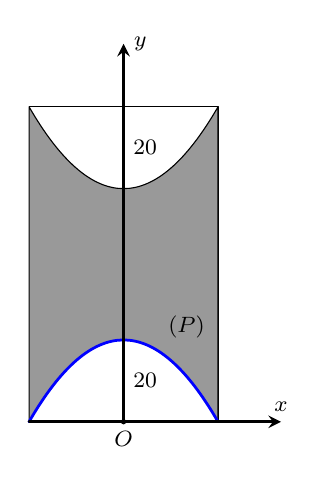
\begin{tikzpicture}[line join = round, line cap=round,>=stealth,font=\footnotesize,scale=0.8]
                \draw (0,0) rectangle (3,5);
                \draw[fill=black!40] (0,0)..controls +(60:2) and +(120:2)..(3,0)--(3,5)
                ..controls +(-120:2) and +(-60:2).. (0,5)--cycle
                ;
                \draw[blue,line width=1pt] (0,0)..controls +(60:2) and +(120:2)..(3,0);
                \draw (2.5,1.5)node[]{$(P)$};
                \draw[] (1.5,0)--(1.5,1.3)node[right,pos=0.5]{$20$};
                \draw[] (1.5,5)--(1.5,3.7)node[right,pos=0.5]{$20$};
                
                \draw[->,line width=1pt] (1.5,0)--(1.5,6)node[right]{$y$};
                \draw[->,line width=1pt] (0,0)--(4,0)node[above]{$x$};
                \fill (1.5,0) circle(1.2pt) node[below]{$O$};
            \end{tikzpicture}
        }
    }
\end{ex}

%%==========Câu 21
\begin{ex}%[Đề Minh Hoạ TNTHPT 2024-2025]%[2PhatTrien-DMH-2024-2025, GV: Hoàng Trọng Tấn]%[id6]
    Một doanh nghiệp dự định sản xuất không quá $500$ sản phẩm. Nếu doanh nghiệp sản xuất $x$ sản phẩm ($1 \leq x \leq 500$) thì doanh thu nhận được khi bán hết số sản phẩm đó là $F(x) = x^3 - 1\,999x^2 + 1\,001\,000x + 250\,000$ đồng, trong khi chi phí sản xuất bình quân cho một sản phẩm là $G(x) = x + 1\,000 + \dfrac{250\,000}{x}$ (đồng). Doanh nghiệp cần sản xuất bao nhiêu sản phẩm để lợi nhuận thu được là lớn nhất?
    \shortans[]{$333$}
    \loigiai{
        Chi phí sản xuất cho $x$ sản phẩm là $xG(x)=x^2+1\,000x+250\,000$ (đồng).
        \\
        Lợi nhuận thu được $L(x)=F(x)-xG(x)= x^3-2\,000x^2+1\,000\,000x$ (đồng).
        \\
        Đạo hàm $L'(x)=3x^2-4\,000x+1\,000\,000$, giải phương trình $L'(x)=0$
        \\
        $3x^2-4\,000x+1\,000\,000=0\Leftrightarrow x=1000$ hoặc $x=\dfrac{2\,000}{6}$.
        \\
        Do $1\le x \le 500$ nên $x=\dfrac{2\,000}{6}$.
        \\
        Mà $333<x=\dfrac{2\,000}{6}<334$.
        \\
        Ta có $L(333)=148\, 148\, 037$, $L(334)=148\,147\,704$, $L(1)=998\,001$ và $L(500)=125\,000\,000$.
        \\
        Vậy doanh nghiệp cần sản xuất $333$ sản phẩm để lợi nhuận thu được là lớn nhất.
    }
\end{ex}

%%==========Câu 22
\begin{ex}%[Đề Minh Hoạ TNTHPT 2024-2025]%[2PhatTrien-DMH-2024-2025, GV: Hoàng Trọng Tấn]%[id6]
    Có hai chiếc hộp, hộp I có $6$ quả bóng màu đỏ và $4$ quả bóng màu vàng, hộp II có $7$ quả bóng màu đỏ và $3$ quả bóng màu vàng, các quả bóng có cùng kích thước và khối lượng. Lấy ngẫu nhiên một quả bóng từ hộp I bỏ vào hộp II. Sau đó, lấy ra ngẫu nhiên một quả bóng từ hộp II. Tính xác suất để quả bóng được lấy ra từ hộp II là quả bóng được chuyển từ hộp I sang, biết rằng quả bóng đó có màu đỏ (làm tròn kết quả đến hàng phần trăm).
    \shortans[]{0,21}
    \loigiai{
        Gọi $A$ là biến cố \lq\lq  quả lấy ra ở II là quả bóng được đưa từ I vào\rq\rq.
        \\
        Gọi $B$ là biến cố \lq\lq  quả bóng lấy ra ở II là đỏ\rq\rq.
        \\
        $\mathrm{P}(B)$ xảy ra theo $2$ trường hợp:
        \\
        \textbf{TH1:} Chuyển một quả đỏ từ I sang II xác suất trường hợp này là $\dfrac{6}{10}\cdot \dfrac{8}{11}$.
        \\
        \textbf{TH2:} Chuyển một quả vàng từ I sang II xác suất trường hợp này là $\dfrac{4}{10}\cdot \dfrac{7}{11}$.
        \\
        Suy ra $\mathrm{P}(B)=\dfrac{6}{10}\cdot \dfrac{8}{11}+\dfrac{4}{10}\cdot \dfrac{7}{11}=\dfrac{38}{55}$.
        \\
        $A\cap B$ là biến cố \lq\lq  quả bóng lấy ra ở II là đỏ và nó là quả bóng thuộc I\rq\rq.
        \\
        Phép thử gồm $2$ hành động: lấy $1$ quả ở I đưa vào II và từ II lấy $1$ quả.
        \\
        Không gian mẫu có $10\cdot 11=110$ kết quả.
        \\
        $A\cap B$ có số kết quả thuận lợi là $6\cdot 1=6$ kết quả.
        \\
        Suy ra $\mathrm{P}(A\cap B)=\dfrac{6}{110}$.
        \\
        Theo định lý Bayes ta có $\mathrm{P}(A\mid B)=\dfrac{\mathrm{P}(A\cap B)}{\mathrm{P}(B)}=\dfrac{\dfrac{6}{110}}{\dfrac{38}{55}}\approx 0{,}08$.
    }
\end{ex}
\Closesolutionfile{ans}
\Closesolutionfile{ansbook}
\inputansbox{6,2,3}{ans/ans-DE-PNL-01-T,ans/ans-DE-PNL-01-TF,ans/ans-DE-PNL-01-SA}

